\documentclass{article}
\usepackage[utf8]{inputenc}
\usepackage{graphicx}

\title{Relazione rapporto e-m elettrone}
\author{Francesco Pio Merafina, Onofrio Davide Caputo, Alessandro Lamesta}
\date{}
\begin{document}
\maketitle
\section{Abstract:}
L'esperimento in questione è una replica dell'esperienza di Thomson per la misura del rapporto carica massa dell'elettrone.
~
\section{Cenni teorici:}
Sappiamo che l'elettrone, essendo carico, è soggetto alla forza di Lorentz, quindi può essere deflesso con un campo magnetico \textbf{B}, o ancora, possiamo calibrare i campi \textbf{E} e \textbf{B} tali che la forza di Lorentz sia nulla, quindi usando la forza di Lorentz nella seconda legge della dinamica possiamo ottenere il rapporto carica massa dell'elettrone. Nel nostro caso abbiamo usato tutte e due le configurazioni.
~
\section{Apparato sperimentale:}
L'apparato sperimentale consiste in un tubo di Thomson, nel quale è stato praticato il vuoto, con all'interno una electron gun; cioè un apparecchio che emette elettroni per effetto termoionico con delle piastre con una d.d.p. acceleratrice degli elettroni, ai lati sono poste delle bobine di Helmotz poste in maniera tale da poter creare un campo \textbf{B} omogeneo nel quale si muove l'elettrone. Si misura la corrente delle bobine mediante un amperometro in serie. Per la misura del raggio di curvatura si utilizza un quadrato tarato in cm di lunghezza 8 cm posto con la diagonale parallela alla traiettoria del fascio di elettroni. Per alimentare il tutto sono stati utilizzati due generatori di tensione. Le bobine hanno un raggio di 6.8cm.
~
\section{Metodologia di misura:}
Per la misura sono state utilizzate due procedure: una in cui il campo \textbf{B} deflette l'elettrone ed una in cui il campo \textbf{B} compensa il campo \textbf{E} ottenendo una traiettoria rettilinea. Una premessa importante va fatta sulla posizione delle bobine, le quali per restituire un campo \textbf{B} il più omogeneo possibile richiedono di essere poste ad una distanza uguale al loro raggio, ma nel nostro caso sono state poste ad una distanza diversa, andando a modificare il coefficente k di proporzionalità tra \textbf{B} ed I.
\subsection{Campo \textbf{B} deflettente:}
In questa configurazione fissiamo la d.d.p. acceleratrice degli elettroni e variamo la corrente che scorre nelle bobine, avendo parametrizzato la relazione tra la corrente I nelle bobine ed il raggio di curvatura, mediante due parametri u e v, abbiamo che il coefficente di proporzionalità tra u e v è il reciproco del rapporto carica massa. Il tutto è stato eseguito a diversi valori fissati di d.d.p. acceleratrice. In questa configurazione si è fatto variare a step di 0.2 cm la posizione x del fascio, fino a quando non si era più in grado di apprezzare la posizione, e si è osservato il valore di corrente I corrispondente a quella posizione.
Le grandezze sulle quali si deve stimare l'incertezza sono la tensione acceleratrice U$_{A}$, la corrente delle bobine I e la deflessione del fascio x. Per la tensione, il cui valore si legge direttamente dal generatore si è stimata una incertezza di 100V, per la corrente, che viene misurata dal tester, si è assunto una incertezza 0.01A, mentre per la x si è assunto una incertezza di 0.01cm. Un altro parametro del quale si deve stimare l'incertezza, ma in questo caso parliamo di incertezza relativa, è il parametro k; il parametro k è stato misurato mediante una sonda Hall, l'incertezza stimata di k è del 5$\%$
\subsection{Campo \textbf{B} compensatore:}
In questa configurazione utilizziamo un campo \textbf{E} perpendicolare a \textbf{B} in modo tale che la forza di Lorentz sia nulla, a fissata d.d.p. acceleratrice, il cui valore si legge direttamente dal generatore. In questa maniera otteniamo una relazione di tipo lineare tra la corrente nelle bobine  e la tensione del condensatore che genera il campo \textbf{E}, dalla pendenza possiamo poi ottenere il rapporto carica massa. Il valore della d.d.p. che genera il campo \textbf{E} è letto dal generatore, ed il tester si usa in serie alle bobine per poter leggere i valori di corrente; facendo variare a step di 100V la d.d.p. osserviamo la variazione di I. 
Le grandezze sulle quali va misurata l'incertezza sono: la corrente I alla quale associamo 0.01A, la tensione acceleratrice U$_{A}$ con incertezza 100V, e la tensione che genera il campo \textbf{E} U$_{p}$ alla quale associamo 1V.
~
\section{Analisi dati:}
Di seguito si riportano tutte le formule teoriche di riferimento per poter eseguire l'esperimento:
\subsection{Campo \textbf{B} deflettente:}
\begin{figure}[h!]
    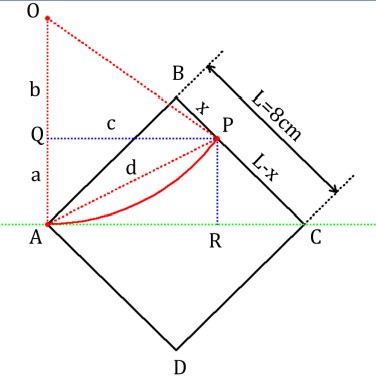
\includegraphics[width=\linewidth]{Rapporto carica-massa.jpg} 
    \caption{Schema di riferimento per la misura del raggio di deflessione del fascio di elettroni}
    \label{figura1}
\end{figure}
Campo Magnetico:
\begin{equation}
    \textbf{B}=\frac{\mu_{0}IR_{b}^2}{2(R_{b}^2 + x^2)^\frac{3}{2}}=kI
\end{equation}
Nel nostro caso x è diverso dal raggio delle bobine R$_{b}$, in particolare vale x=9cm.

Forza di Lorentz:
\begin{equation}
    F=-e(\textbf{v} \times \textbf{B})
\end{equation}
Conservazione dell'energia:
\begin{equation}
    \frac{1mv^2}{2}=eU_{A}
\end{equation}
Raggio di curvatura in funzione della deflessione:
\begin{equation}
    R=\frac{L^2 + x^2}{(L-x)\sqrt{2}}
\end{equation}
Rapporto carica massa:
\begin{equation}
    \frac{e}{m}=\frac{4U_{A}(L-x))^2}{k^2I^2(L^2+x^2)^2}
\end{equation}
Riparametrizzazione:
\begin{equation}
    u=k^2I^2(L^2+x^2)^2;
    v=4U_{A}(L-x))^2
\end{equation}
Rapporto carica massa:
\begin{equation}
    u=\frac{v}{\frac{e}{m}}
\end{equation}

\subsection{Campo \textbf{B} compensatore:}
Forza di Lorentz:
\begin{equation}
    F=-e(\textbf{E}+\textbf{v} \times \textbf{B})
\end{equation}
Campo Elettrico:
\begin{equation}
    E=\frac{U_{P}}{d}
\end{equation}
Rapporto carica massa:
\begin{equation}
    \frac{e}{m}=(\frac{E}{B})^2\frac{1}{2U_{A}}=(\frac{U_{P}}{dkI})^2\frac{1}{2U_{A}}
\end{equation}
Relazione pendenza retta di fit con rapporto carica massa:
\begin{equation}
    \frac{e}{m}=\frac{\alpha^2}{2U_{A}(kd)^2}
\end{equation}
dove $\alpha$ è la pendenza della retta di fit.
~
\section{Risultati e conclusioni:}
Tratteremo separatamente i risultati delle due metodologie di misura:
\subsection{Campo \textbf{B} deflettente:}
Osservando il grafico in figura 2, ottenuto con i dati della tabella  1 otteniamo un risultato del rapporto carica massa di:
$\frac{e}{m}$=(1.56±0.09)*10$^{11}$ C*kg$^{-1}$ con un rapporto tra valore misurato e valore vero del 88$\%$
\subsection{Campo \textbf{B} compensatore:}
Osservando il grafico in figura 3, ottenuta con la tabella 2, otteniamo un rapporto carica massa di: $\frac{e}{m}$=(6.18±0.50)*10$^{11}$ C*kg$^{-1}$, molto diverso da quello vero, questo può essere imputabile a due fattori: una oggettiva difficoltà operativa nella rettificazione del fascio, ed una costante di proporzionalità tra campo magnetico e corrente nelle bobine molto diversa da quella indicata.
~
\section{Grafici:}
\begin{figure}[h!]
    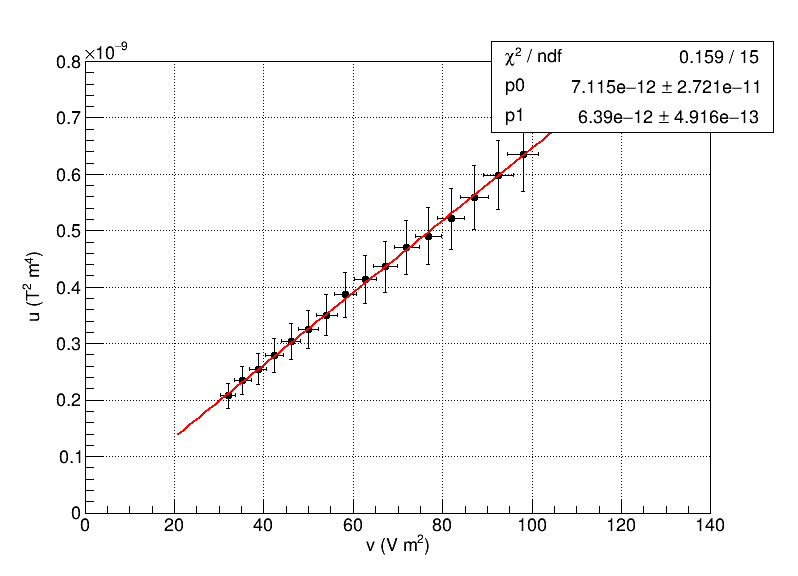
\includegraphics[width=\linewidth]{5000.png} 
    \caption{Grafico del parametro u in funzione del parametro v con valore di U$_{A}$=5000V}
    \label{figura1}
\end{figure}
\begin{figure}[h!]
    \includegraphics[width=\linewidth]{e_m.png} 
    \caption{Grafico campo magnetico compensante, con tensione U$_{A}$=5000V}
    \label{figura1}
\end{figure}
\end{document}